\documentclass[tikz,border=6pt]{standalone}
\usepackage{amsmath}
\usetikzlibrary{arrows.meta,positioning,backgrounds,fit,calc}

\begin{document}
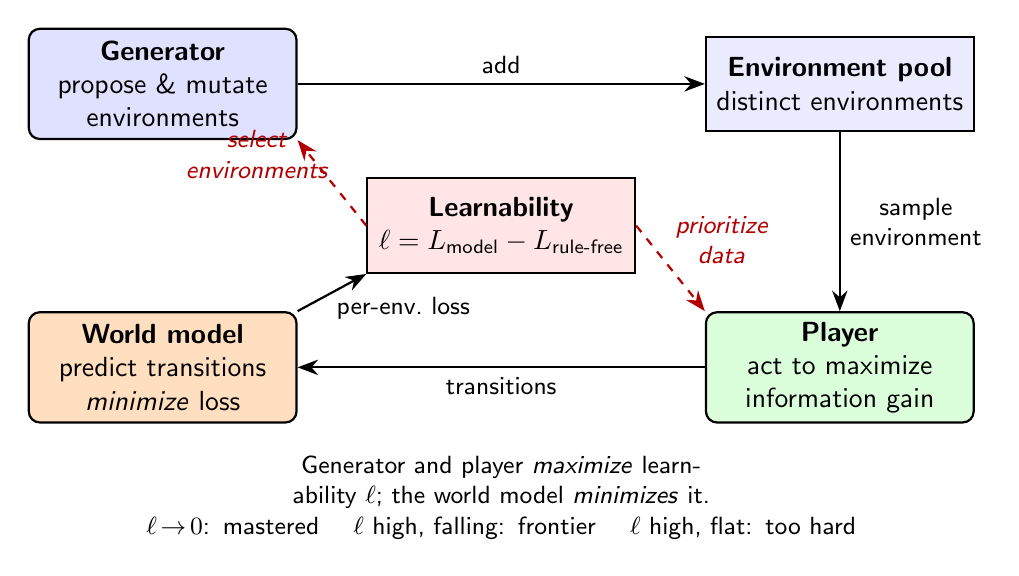
\begin{tikzpicture}[
  font=\sffamily,
  >={Stealth[length=2.6mm]},
  proc/.style={draw,rounded corners,thick,align=center,
               minimum width=34mm,minimum height=14mm,fill=#1},
  store/.style={draw,thick,align=center,fill=#1,
                minimum width=34mm,minimum height=12mm},
  flow/.style={->,thick},
  steer/.style={->,thick,red!70!black,dashed},
  lbl/.style={font=\sffamily\small,align=center},
  slbl/.style={font=\sffamily\small\itshape,align=center,red!70!black},
]

% --- nodes: forward cycle on the outer rectangle, signal at the hub ---
\node[proc=blue!12]   (gen)  at (0  ,3.6) {\textbf{Generator}\\propose \& mutate\\environments};
\node[store=blue!8]   (pool) at (8.6,3.6) {\textbf{Environment pool}\\distinct environments};
\node[proc=green!14]  (play) at (8.6,0  ) {\textbf{Player}\\act to maximize\\information gain};
\node[proc=orange!25] (wm)   at (0  ,0  ) {\textbf{World model}\\predict transitions\\\emph{minimize} loss};
\node[store=red!10]   (sig)  at (4.3,1.8) {\textbf{Learnability}\\$\ell=L_{\text{model}}-L_{\text{rule-free}}$};

% --- forward data cycle (outer rectangle) ---
\draw[flow] (gen)  -- node[lbl,above]{add} (pool);
\draw[flow] (pool) -- node[lbl,right]{sample\\environment} (play);
\draw[flow] (play) -- node[lbl,below]{transitions} (wm);

% --- the hub: model emits the signal it tries to crush; signal steers the maximizers ---
\draw[flow]  (wm.north east)  -- node[lbl,below right=-1mm]{per-env.\ loss} (sig.south west);
\draw[steer] (sig.west) -- node[slbl,above left=-1mm]{select\\environments} (gen.south east);
\draw[steer] (sig.east) -- node[slbl,above right=-1mm]{prioritize\\data} (play.north west);

% --- legend ---
\node[lbl, below=10mm of $(wm)!0.5!(play)$, text width=92mm]
  {Generator and player \emph{maximize} learnability $\ell$; the world model \emph{minimizes} it.\\
   $\ell\!\to\!0$: mastered \quad $\ell$ high, falling: frontier \quad $\ell$ high, flat: too hard};

\end{tikzpicture}
\end{document}
